\documentclass[Arkitektur/System_main.tex]{subfiles}
\begin{document}
\subsubsection{Oprettelse af bruger profil}
For at kunne bruge funktionalitetterne i CarnGo applikationen er at lave en bruger profil.Til at beskrive denne funktionalitet er der lavet et sekvensdiagram, der beskriver samspillet mellem lejer/udlejer, applikation og database. Udover dette er der også lavet en applikationsmodel. Sekvensdiagrammet ses på figur \ref{fig:UserSignUpSD}.
\begin{figure}[H]
    \centering
    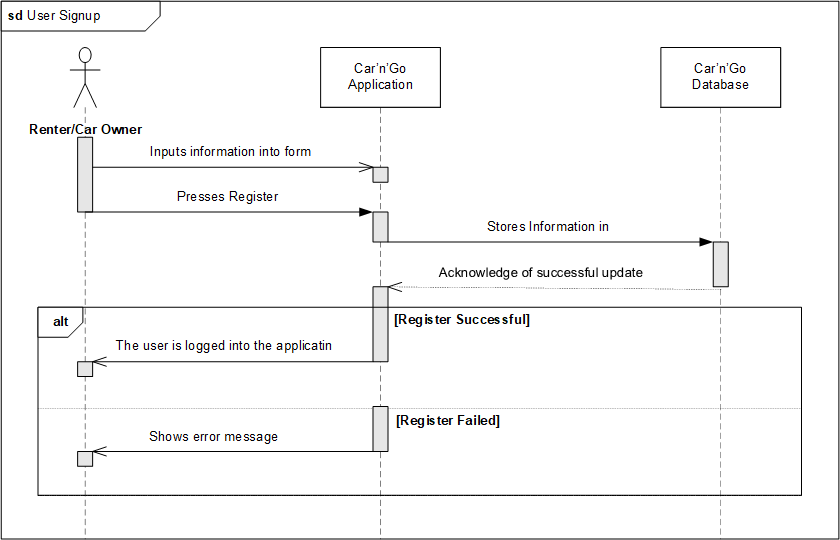
\includegraphics[width=\textwidth]{Arkitektur/Softwarearkitektur/User_Signup/graphics/UserSignupSD.png}
    \caption{Her ses et skevens diagram for samspillet mellem lejer/udlejer, CarnGo Applikationen samt databasen.}
    \label{fig:UserSignUpSD}
\end{figure}

Applikationsmodellen består af et klassediagram, samt et statemachine diagram. Klassediagrammet ses på figur \ref{fig:UserSignUpCD} og statemchine diagrammet MANGLER.
\begin{figure}[H]
    \centering
    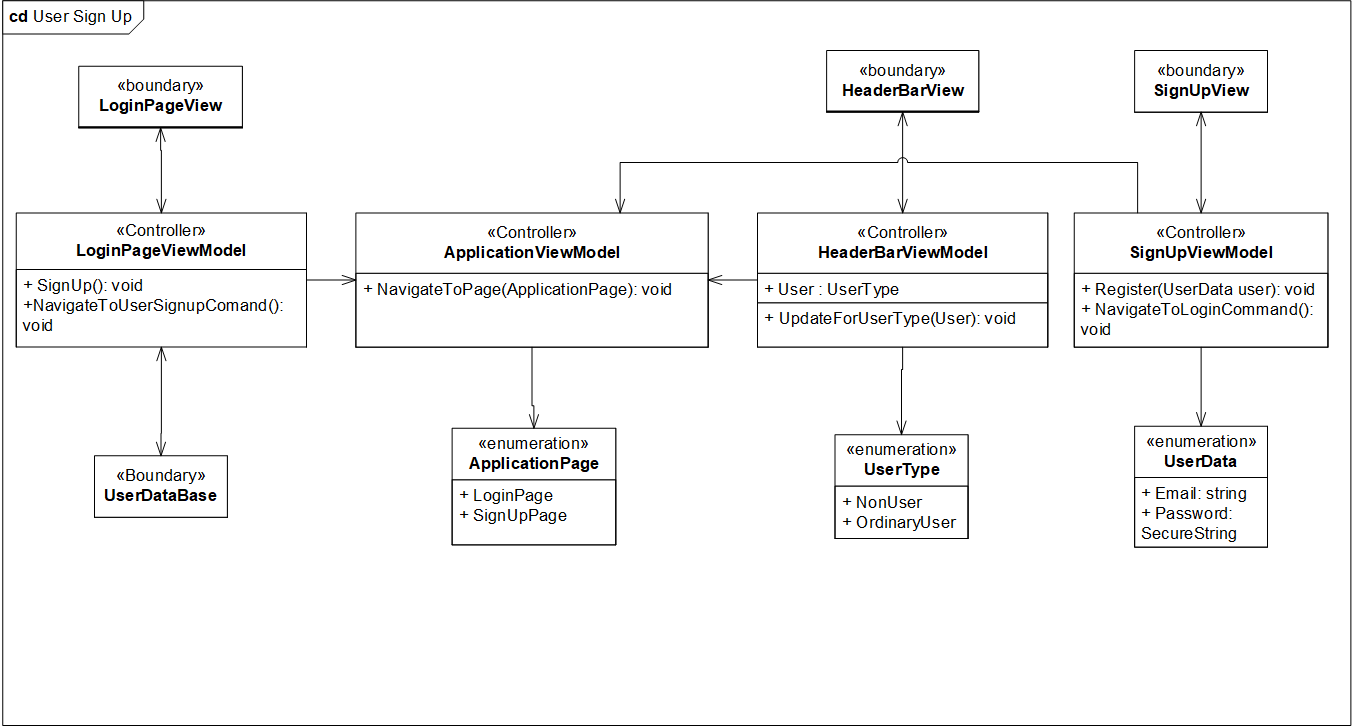
\includegraphics[width=\textwidth]{Arkitektur/Softwarearkitektur/User_Signup/graphics/UserSignUpCD.png}
    \caption{Klassediagram for oprettelse af bruger profil. }
    \label{fig:UserSignUpCD}
\end{figure}
EN MANGLENDE STATEMACHINE?



\end{document}